\documentclass[tikz, border=10pt]{standalone}
\usepackage{tikz}
\usetikzlibrary{shapes.multipart, positioning, arrows.meta, calc}

\begin{document}
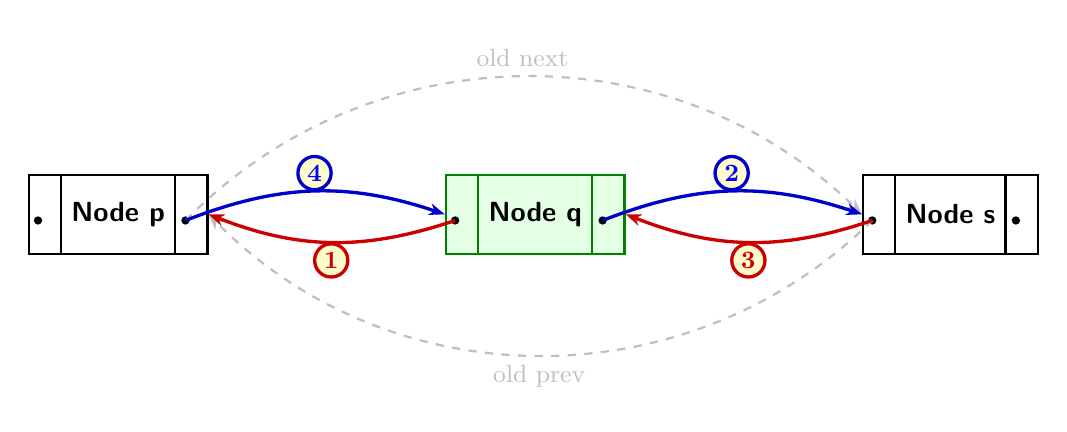
\begin{tikzpicture}[
    dblnode/.style={
        rectangle split,
        rectangle split parts=3,
        rectangle split horizontal,
        draw,
        thick,
        fill=white,
        minimum height=1cm,
        rectangle split part fill={white, white, white},
        font=\sffamily
    },
    newnode/.style={
        dblnode,
        fill=green!10,
        draw=green!50!black,
        rectangle split part fill={green!10, green!10, green!10}
    },
    ptr/.style={
        >={Stealth[length=2mm]},
        ->,
        thick,
        blue
    },
    revptr/.style={
        >={Stealth[length=2mm]},
        ->,
        thick,
        red!80!black
    },
    oldptr/.style={
        ptr,
        dashed,
        gray!50
    },
    oldrevptr/.style={
        revptr,
        dashed,
        gray!50
    },
    newptr/.style={
        ptr,
        draw=blue!80!black,
        very thick
    },
    newrevptr/.style={
        revptr,
        draw=red!80!black,
        very thick
    },
    stepmarker/.style={
        font=\small\bfseries,
        circle,
        draw,
        fill=yellow!20,
        inner sep=1pt,
        minimum size=12pt
    }
]

    % Nodes
    \node[dblnode] (nodeP) { \nodepart{one} \phantom{x} \nodepart{two} \textbf{Node p} \nodepart{three} \phantom{x}};
    
    % Node Q (New) placed below between P and S initially, or just between them with more spacing
    % Let's place Q in the middle but vertically offset to make the cross-linking clear?
    % The user's mermaid suggests P - Q - S in a line, but originally P - S.
    % Let's place P and S far apart, and Q in the middle.
    
    \node[newnode, right=3cm of nodeP] (nodeQ) { \nodepart{one} \phantom{x} \nodepart{two} \textbf{Node q} \nodepart{three} \phantom{x}};
    
    \node[dblnode, right=3cm of nodeQ] (nodeS) { \nodepart{one} \phantom{x} \nodepart{two} \textbf{Node s} \nodepart{three} \phantom{x}};

    % Dots in pointer fields
    \fill[black] (nodeP.one) circle (1.5pt);
    \fill[black] (nodeP.three) circle (1.5pt);
    \fill[black] (nodeQ.one) circle (1.5pt);
    \fill[black] (nodeQ.three) circle (1.5pt);
    \fill[black] (nodeS.one) circle (1.5pt);
    \fill[black] (nodeS.three) circle (1.5pt);


    % 0. Old links (P <-> S) - These are logically "before", likely pointing to each other.
    % Current visualization: P -> S and S -> P directly, but now obscured by Q or passing through.
    % We'll draw them curved high/low to represent the "old" state being replaced.
    
    \draw[oldptr] (nodeP.three) to[bend left=45] node[midway, above] {\small old next} (nodeS.west);
    \draw[oldrevptr] (nodeS.one) to[bend left=45] node[midway, below] {\small old prev} (nodeP.east);

    
    % New Pointers with steps
    
    % 1. Q.prev -> P
    % From Q.one to P.east (or P node)
    \draw[newrevptr] (nodeQ.one) to[bend left=20] node[midway, below, stepmarker] {1} (nodeP.east);
    
    % 2. Q.next -> S
    % From Q.three to S.west
    \draw[newptr] (nodeQ.three) to[bend left=20] node[midway, above, stepmarker] {2} (nodeS.west);
    
    % 3. S.prev -> Q
    % From S.one to Q.east/Q node
    \draw[newrevptr] (nodeS.one) to[bend left=20] node[midway, below, stepmarker] {3} (nodeQ.east);
    
    % 4. P.next -> Q
    % From P.three to Q.west
    \draw[newptr] (nodeP.three) to[bend left=20] node[midway, above, stepmarker] {4} (nodeQ.west);

    % Optional: Labels for steps?
    % User provided: sequence 4-1-2-3 in mermaid?
    % Mermaid:
    % P -- "4" --> Q
    % Q -- "1" --> P
    % Q -- "2" --> S
    % S -- "3" --> Q
    % Just following the numbers from the user request.
    
\end{tikzpicture}
\end{document}
